\documentclass{article}
\usepackage[top=1cm, left=1.5cm, right=1.5cm, bottom=1.5cm]{geometry}
\usepackage{graphicx, amsmath, tikz-cd, apacite, amssymb, tcolorbox, wrapfig}
\graphicspath{{./img/}}
\bibliographystyle{apacite}
\setlength{\parindent}{0pt}
\setlength{\parskip}{1em} 

\title{Independencia Lineal}
\author{Pablo Darío}
\date{02/01/2023}
 
\begin{document}
\maketitle
Las ecuaciones homogéneas se pueden estudiar desde una perspectiva diferente si las escribimos como ecuaciones vectoriales. De esta manera, la atención se transfiere de las soluciones desconocidas de $A\mathbf{x} = 0$ a los vectores que aparecen en las ecuaciones vectoriales.

Por ejemplo, considere la ecuación 

\begin{equation*}
    x_1\begin{bmatrix} 1\\2\\3 \end{bmatrix}
    + x_2\begin{bmatrix} 4\\5\\6 \end{bmatrix}
    + x_3\begin{bmatrix} 2\\1\\0 \end{bmatrix}
    = \begin{bmatrix} 0\\0\\0 \end{bmatrix}
\end{equation*}

Esta ecuación tiene una solución trivial, desde luego, donde $x_1 = x_2 = x_3 = 0$.

\begin{tcolorbox}[colback=blue!10!white,colframe=blue!60!black,title=Independencia Lineal]
    Se dice que un conjunto indexado de vectores \{$\mathbf{v_1},..., \mathbf{v_p}$\} en $\mathbb{R}^n$ es linealmente independiente si la ecuación vectorial $$x_1\mathbf{v_1} + x_2\mathbf{v_2} + ... + x_p\mathbf{v_p} = 0$$
    solo tiene la solución trivial. Se dice que el conjunto \{$\mathbf{v_1},..., \mathbf{v_p}$\} es linealmente dependiente si existen pesos $c_1, ..., c_p$ no todos cero, tales que $$c_1\mathbf{v_1} + c_2\mathbf{v_2} + ... + c_p\mathbf{v_p} = 0$$
\end{tcolorbox}

La última ecuación se llama relación de dependencia lineal entre $\mathbf{v_1},..., \mathbf{v_p}$ cuando no todos los pesos son cero. Un conjunto indexado es linealmente dependiente si y solo si no es linealmente independiente. Por brevedad, puede decirse que $\mathbf{v_1},..., \mathbf{v_p}$ son linealmente dependientes cuando queremos decir que \{$\mathbf{v_1},..., \mathbf{v_p}$\} es un conjunto linealmente dependiente. Se utiliza una 
terminología semejante para los conjuntos linealmente independientes.

\begin{large}
    \textbf{Ejemplo}
\end{large}

Sean $\mathbf{v_1} = \begin{bmatrix} 1\\2\\3\end{bmatrix}, \mathbf{v_2} = \begin{bmatrix} 4\\5\\6 \end{bmatrix} \text{ y } \mathbf{v_1} = \begin{bmatrix} 2\\1\\0 \end{bmatrix}$

Determine si el conjunto \{$\mathbf{v_1},\mathbf{v_2}, \mathbf{v_3}$\} es linealmente independiente 

Se debe determinar si existe una solución no trivial. Reduciendo a la matriz a su forma escalonada, obtenemos:

\begin{equation*}
    \left[\begin{array}{rrr|r}
    1 & 4 & 2 & 0 \\
    2 & 5 & 1 & 0 \\
    3 & 6 & 0 & 0
    \end{array}\right] \sim\left[\begin{array}{rrr|r}
    1 & 4 & 2 & 0 \\
    0 & -3 & -3 & 0 \\
    0 & 0 & 0 & 0
    \end{array}\right]
\end{equation*}

Por lo tanto $x_1$ y $x_2$ son variables básicas y $x_3$ es libre. Cada valor de $x_3$ distinto determina una solución no trivial. Así que $\mathbf{v_1}, \mathbf{v_2}, \mathbf{v_3}$ son \textbf{linealmente dependientes} (por tanto no son linealmente independientes).

\pagebreak

Para encontrar una \textbf{relación de dependencia lineal} entre $\mathbf{v_1}, \mathbf{v_2}, \mathbf{v_3}$ se reduce por filas completamente a la matriz aumentada y se escribe el nuevo sistema:

\begin{equation*}
    \begin{aligned}
        x_1 & & -2x_3 &= 0\\
        & x_2 & +x_3 &=0\\
        & & 0 &= 0
    \end{aligned}
\end{equation*}

Así $x_1 = 2x_3, x_2 = -x_3$ y $x_3$ es libre. Seleccione cualquier valor distinto de cero para $x_3$; por ejemplo $x_3 = 5$. De esta manera obtenemos la \textbf{relación de dependencia lineal:}$$10\mathbf{v_1} - 5\mathbf{v_2} + 5\mathbf{v_3}=0$$

Esta es una (entre una infinidad) de las posibles relaciones de dependencia lineal entre $\mathbf{v_1}, \mathbf{v_2}, \mathbf{v_3}$

\begin{tcolorbox}[colback=blue!10!white,colframe=blue!60!black,title=Columnas de una Matriz]
    Las columnas de una matriz $A$ son linealmente independientes si y solo si la ecuación $A\mathbf{x} = 0$ tiene solo la solución trivial.
\end{tcolorbox}

Así bien si tenemos una matriz $A = \begin{bmatrix} a_1 & \dotsb & a_n \end{bmatrix}$, la ecuación matricial  $A\mathbf{x} = 0$ se puede escribir como $$x_1\mathbf{a_1} + x_2\mathbf{a_2} + ... + x_n\mathbf{a_n} = 0$$

Cada relación de dependencia lineal entre las columnas de $A$ corresponde a una solución no trivial de $A\mathbf{x} = 0$.

\begin{large}
    \textbf{Ejemplo}
\end{large}

Determine si las columnas de la matriz $A = \begin{bmatrix}
    0 & 1 & 4\\
    1 & 2 & -1\\
    5 & 8 & 0
\end{bmatrix}$ son linealmente independientes.

Se reduce por filas la matriz aumentada:

\begin{equation*}
    \left[\begin{array}{rrr|r}
        1 & 2 & -1 & 0 \\
        0 & 1 & 4 & 0 \\
        0 & 0 & 13 & 0
        \end{array}\right]
\end{equation*}

En este punto está claro que hay 3 variables básicas y ninguna variable libre. Así la ecuación $A\mathbf{x} = 0$ solo tiene la solución trivial y las columnas de $A$ son \textbf{linealmente independientes}.

\begin{large}
    \textbf{Conjuntos de uno o dos vectores}
\end{large}

Un conjunto que solo tiene un vector $\mathbf{v}$ es linealmente independiente si y solo si $\mathbf{v}$ no es el vector cero. Esto se debe a que la ecuación vectorial $x_1\mathbf{v} = 0$ solo tiene la solución trivial cuando $\mathbf{v} \neq 0$. El vector cero es linealmente dependiente porque $x_{1}0=0$
tiene muchas soluciones no triviales.

\begin{large}
    \textbf{Ejemplo}
\end{large}

Determine si los siguientes conjutnos de vectores son linealmente independientes

\begin{equation*}
    \mathbf{v_1} = \begin{bmatrix} 3\\1  \end{bmatrix},
    \mathbf{v_2} = \begin{bmatrix} 6\\2  \end{bmatrix}
\end{equation*}

Podemos observar que $\mathbf{v_2}$ es múltiplo de $\mathbf{v_1}$, para ser exactos $\mathbf{v_2} = 2\mathbf{v_1}$. Así que $-2\mathbf{v_1} + \mathbf{v_2}= 0$, lo que demuestra que \{$\mathbf{v_1}, \mathbf{v_2}$\} es linealmente independiente.

\begin{large}
    \textbf{Ejemplo 2}
\end{large}

\begin{equation*}
    \mathbf{v_1} = \begin{bmatrix} 3\\2  \end{bmatrix},
    \mathbf{v_2} = \begin{bmatrix} 6\\2  \end{bmatrix}
\end{equation*}

Desde luego los vectores $\mathbf{v_1}$ y $\mathbf{v_2}$ no son múltiplos entre sí; por lo tanto \{$\mathbf{v_1}, \mathbf{v_2}$\} es un conjunto linealmente independiente.

\begin{tcolorbox}[colback=red!10!white, colframe=red!70!black, title=Conjunto de 2 vectores]
    Un conjunto de dos vectores \{$\mathbf{v_1}, \mathbf{v_2}$\} es linealmente dependiente si al menos uno de los vectores es un múltiplo del otro. El conjunto es linealmente independiente si y solo si ninguno de los vectores es un múltiplo del otro.
\end{tcolorbox}

En términos geométricos, dos vectores son linealmente dependientes si y solo si ambos están sobre la misma recta que pasa por el origen. 

\begin{figure}[ht]
    \centerline{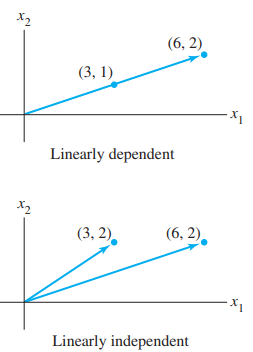
\includegraphics[width=0.3\textwidth]{image14.png}}
    \caption{Dependencia Lineal en $\mathbb{R}^2$}
\end{figure}

\begin{tcolorbox}[colback=blue!10!white,colframe=blue!60!black,title=Caracterización de conjuntos linealmente dependientes]
    Un cojunto de dos o más vectores es linealmente dependiente si y solo si al menos uno de los vectores en el conjunto es una combinación lineal de los otros. De hecho si el conjunto es linealmente dependiente y $\mathbf{v_1} \neq 0$ entonces alguna $\mathbf{v_j}$ (con $j > 1$) es una combinación lineal de los vectores precedentes $v_1, \dotsb, v_{j-1}$
\end{tcolorbox}

\begin{figure}[ht]
    \centerline{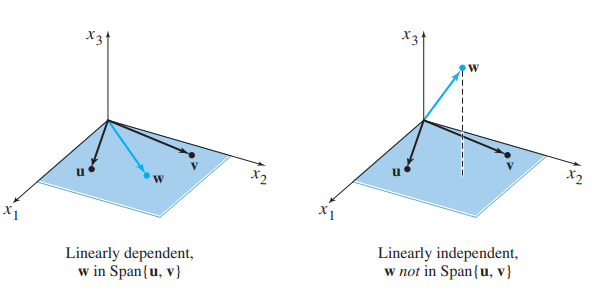
\includegraphics[width=0.3\textwidth]{image15.png}}
    \caption{Dependencia Lineal en $\mathbb{R}^3$}
\end{figure}

\begin{tcolorbox}[colback=red!10!white, colframe=red!70!black, title=Caso Especial]
    Si un conjunto contiene más vectores que entradas en cada vector, entonces el conjutno es linealmente dependiente. Es decir, cualquier conjunto \{$\mathbf{v_1}, \dotsb, \mathbf{v_p}$\} en $\mathbb{R}^n$ es linealmente dependiente si $p > n$. 
    Ya que si $p > n$, entonces hay mas variables que ecuaciones, por lo que debe de quedar una variable libre al menos.
\end{tcolorbox}

\begin{tcolorbox}[colback=red!10!white, colframe=red!70!black, title=Caso especial 2]
    Si un conjunto de vectores contiene al vector cero, entonces el conjunto es linealmente dependiente.
\end{tcolorbox}

Al remunerar los vectores, se puede suponer que $\mathbf{v_1} = 0$. Así la ecuación $1\mathbf{v_1} + 0\mathbf{v_2} + \dotsb + 0\mathbf{v_p} = 0$ indica que el conjunto es linealmente dependiente, ya que se le pueden asignar infinitos pesos a $x_1$ que al multiplicarse por $\mathbf{v_1}$ (el vector cero), dará siempre cero y la suma de todos los vectores con la condición anterior será 0 para todas las entradas. \cite{DavidC}

\begin{tcolorbox}[colback=red!10!white, colframe=red!70!black, title=Resumen]
    La dependencia lineal de dos vectores en $\mathbb{R}^2$ se puede visualizar como dos vectores colindantes en una recta y la Independencia como dos vectores que no colindan en una recta. Para más vectores en $\mathbb{R}^3$ se pueden visualizar como que los vectores están en el mismo plano.
    \begin{itemize}
        \item[-] Un conjunto de vectores es linealmente independiente si la única solución a la ecuación $A\mathbf{x} = 0$ es la trivial, por lo tanto un conjunto de vectores es linealmente dependiente si la ecuación $A\mathbf{x} = 0$ tiene al menos una variable libre o bien si tiene una infinidad de soluciones a parte de la solución trivial.
        \item[-] Un conjunto de vectores es linealmente dependiente si un vector puede ser representado como la combinación lineal de los otros vectores.
        \item[-]  Un conjunto \{$\mathbf{v_1},..., \mathbf{v_p}$\} es linealmente dependiente si existen pesos $c_1, ..., c_p$ donde al menos uno es diferente de cero, tales que $$c_1\mathbf{v_1} + c_2\mathbf{v_2} + ... + c_p\mathbf{v_p} = 0$$
        \item[-] Dos vectores son linealmente dependiente si uno es múltiplo de otro. 
        \item[-] Si hay más vectores que entradas, significa que tenemos más variables que ecuaciones, por lo tanto, alguna variable es libre y el conjunto de vectores el linealmente dependiente. 
        \item[-] Si un conjunto tiene al vector 0, entonces el conjunto es linealmente dependiente, ya que el vector 0 es linealmente dependiente, esto debido a que podemos asignar todos los pesos como 0, excepto el del vector cero $$c_1\mathbf{v_1} + 0\mathbf{v_2} + \dotsb + 0\mathbf{v_p} = 0$$
        \item[-] Un conjunto de un vector es linealmente independiente si y solo si no es el vector cero, ya que un vector no nulo solo tiene la solución trivial.  
    \end{itemize}
\end{tcolorbox}

\bibliography{Referencias}
\end{document}